\section{Snooping protocols}

In snooping protocols, each cache controller snoops the bus to determine if it has a copy of the block requested.
Each cache that holds a copy of the shared block also maintains the status of its sharing independently, without centralized state management.

Requests for shared data are broadcasted to all processors due to the caching information residing in each processor's cache. 
This broadcast mechanism ensures that caches are updated with the latest state of shared data.

Snooping protocols are well-suited for centralized shared memory architectures, particularly in small-scale multiprocessors with a single shared bus. 
This architecture allows efficient coordination and synchronization among caches without the need for centralized control, leveraging the bus as a communication medium for maintaining cache coherence.

\paragraph*{Snoopy cache}
The concept of a Snoopy cache, introduced by Goodman in 1983, revolves around caches actively monitoring DMA transfers and other bus transactions to maintain coherence. 
The core idea is for each cache to do the right thing based on the observed bus transactions.
Snoopy cache tags are designed to be dual-ported, facilitating efficient monitoring of bus transactions without significantly impacting processor performance.
\begin{figure}[H]
    \centering
    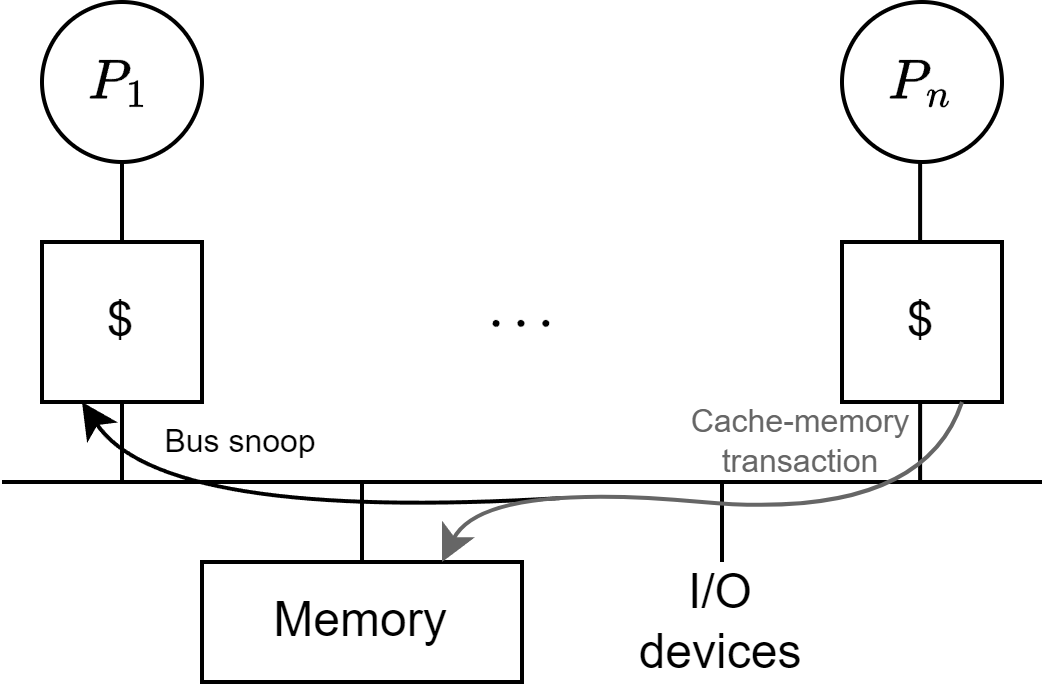
\includegraphics[width=0.5\linewidth]{images/snop.png}
    \caption{Snoopy cache}
\end{figure}
In a Snoopy cache architecture:
\begin{itemize}
    \item The bus serves as a broadcast medium, and each cache maintains awareness of the data it holds.
    \item Cache controllers snoop on all transactions on the shared bus. 
        If a transaction involves a block that a cache contains, the cache controller takes action to maintain coherence—such as invalidating, updating, or supplying data based on the block's current state and the protocol in use.
\end{itemize}
Due to the frequent checking of cache address tags during bus transactions, interference with processor operations can occur, potentially leading to stalls when the cache is unavailable.

To mitigate interference and maintain processor performance, the address tag portion of the cache is duplicated specifically for snooping activities. 
This duplication typically involves adding an extra read port to the address tag portion of the cache, allowing snooping operations to proceed independently of normal cache accesses.
\begin{figure}[H]
    \centering
    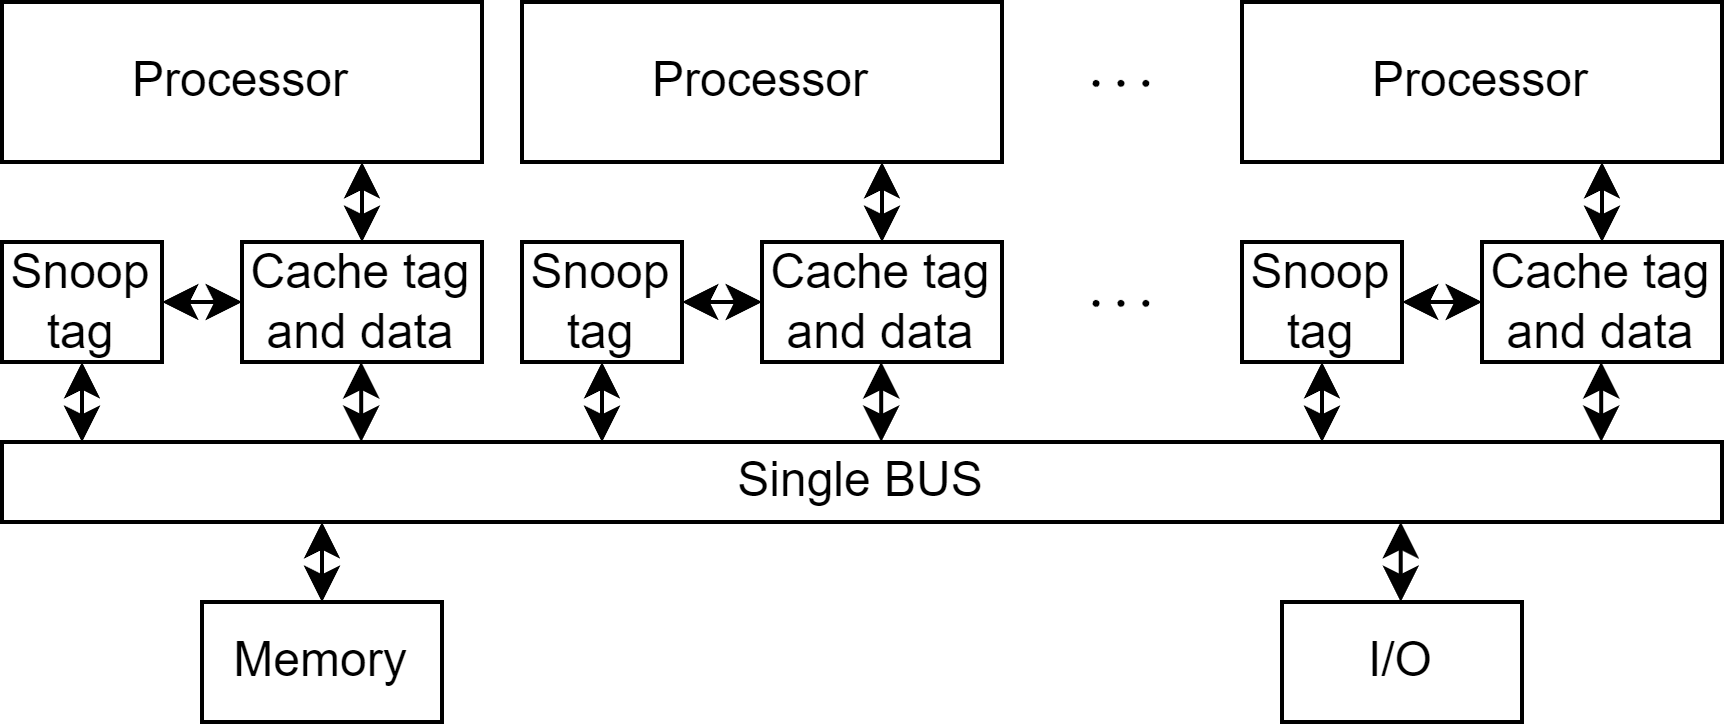
\includegraphics[width=0.75\linewidth]{images/snopt.png}
    \caption{Snoop tag}
\end{figure}
Snooping protocols are categorized based on their handling of write operations:
\begin{itemize}
    \item \textit{Write invalidate protocol}: when a processor writes to a block, all other caches holding copies of that block are invalidated. 
        This ensures that only one copy of the data is active at any given time.
    \item \textit{Write update protocol}: when a processor writes to a block, the updated data is broadcasted to all other caches holding copies of that block. 
        This allows multiple caches to maintain coherent copies of the data.
\end{itemize}

\subsection{Write invalidate protocol}
In the Write Invalidate Protocol, the process of updating data is managed through the following steps:
\begin{enumerate}
    \item The writing processor initiates an invalidation signal over the shared bus, instructing all other caches to invalidate their copies of the data before it modifies its local copy. 
    \item After issuing the invalidation signal, the writing processor is free to update its local data until another processor requests it.
    \item All caches connected to the bus check if they possess a copy of the data. If so, they invalidate the corresponding data block to maintain coherence.
\end{enumerate}
This protocol supports multiple processors reading from the data concurrently but restricts writing to one processor at a time.
Initially, the bus is utilized solely for the first write operation to invalidate other copies. 
Subsequent writes do not require bus activity unless a cache with the data block is accessed.
In case of a read miss:
\begin{itemize}
    \item \textit{Write through}: ensures memory is always updated immediately.
    \item \textit{Write back}: involves snooping in caches to locate the most recent copy of the data.
\end{itemize}

\paragraph*{MESI protocol}
The MESI Protocol governs the state management of cache blocks with four distinct states:
\begin{itemize}
    \item \textit{Modified}: the block is dirty and exclusive to the cache holding it. 
        It cannot be shared, and this cache is the sole holder with writable access.
    \item \textit{Exclusive}: the block is clean, and only one cache has a copy. 
        It is not shared with other caches.
    \item \textit{Shared}: the block is clean, and multiple caches have copies of it.
    \item \textit{Invalid}: the block contains no valid data and is not currently in use.
\end{itemize}
In both the Shared and Exclusive states, the memory holds an up-to-date version of the data.
When a write operation occurs:
\begin{itemize}
    \item Writing to an Exclusive block does not necessitate sending an invalidation signal over the bus because no other caches hold copies of the block.
    \item Writing to a Shared block requires invalidating all other copies of the block in the caches to maintain coherence.
\end{itemize}
The MESI Protocol optimizes cache coherence by efficiently managing the states of cache blocks, ensuring data integrity and minimizing bus traffic in shared-memory architectures.

\subsection{Write update protocol}
In Write update protocol, the writing processor broadcasts new data over the bus. 
Each cache checks if it holds a copy of the data. If a copy exists, it updates all copies with the new value.

This approach necessitates continuous broadcast of write operations to shared data. 
Unlike the write-invalidate protocol, which removes all copies except for a single local copy for subsequent writes, this protocol resembles write-through because all writes propagate over the bus to update shared data copies.

An advantage of this protocol is the reduced latency in caches, as new values appear sooner. 
This ensures that memory is always up-to-date, minimizing read misses.

\subsection{Typical cache configuration}
The majority of commercial cache-based multiprocessors commonly utilize:
\begin{itemize}
    \item \textit{Write-back caches}: these caches reduce bus traffic by allowing multiple processors on a single bus. 
        They use a snooping scheme to determine the most recent data value of a cache block in case of a cache miss. 
        Each processor monitors every address placed on the bus. 
        If a processor discovers it holds a dirty copy of the requested cache block, it responds with that cache block.
    \item \textit{Write invalidate protocol}: this protocol is employed to conserve bus bandwidth. 
        It ensures write serialization due to the bus being a single point of arbitration. 
        Therefore, a write to a shared data item cannot complete until it gains bus access.
\end{itemize}

\subsection{Cache consistency}
\begin{definition}[\textit{System sequential consistency}]
    A system is sequentially consistent if the result of any execution is the same as if the operations of all processors were executed in some sequential order, and the operations of each individual processor appear in the order specified by the program.
\end{definition}
Sequential consistency means that any execution yields the same result as if all processor operations were executed in a specific sequential order, respecting the program's specified order.

In practice, ensuring sequential consistency requires processors to observe data writes from other processors in a particular order. 
This consistency model guarantees that memory accesses from different processors are interleaved in a way that preserves the program's intended order.

To achieve sequential consistency, processors may delay completing memory accesses until all invalidations resulting from those accesses are finished. 
This ensures that all processors see a consistent view of memory at all times.

While maintaining sequential consistency can impact performance, it is typically not a significant issue for most programs that are inherently synchronized or structured to handle such consistency constraints effectively.

\paragraph*{Synchronization}
A program is considered synchronized when all access to shared data is ordered by synchronization operations.
Synchronization becomes necessary whenever concurrent processes exist, even in a uniprocessor system. 
There are two primary classes of synchronization:
\begin{itemize}
    \item \textit{Producer consumer}: a consumer process waits until a producer process has produced data.
    \item \textit{Mutual exclusion}: ensures that only one process can use a resource at any given time.
\end{itemize}

\paragraph*{Locks}
In the Sequential Consistency (SC) model, regular loads and stores (and fences in weaker models) are adequate for implementing mutual exclusion. 
However, this approach can lead to inefficient and complex code. 
As a result, atomic Read Modify Write (RMW) instructions have been introduced into Instruction Set Architectures (ISAs) to support efficient mutual exclusion.